\section{Consultar Tratamientos de Pacientes}

Un doctor tendrá una lista con todos los tratamientos de sus pacientes, tanto los que están en estado activo, incompleto, interrumpido y terminado. De esta manera sabrá cuantos y cuáles son sus tratamientos, su estado y la información de estos, como nombre de tratamiento, paciente al que se le expidió, fecha de expedición y número de medicamentos.

\subsubsection{Procedimiento}
\begin{enumerate}
	
	\item Selecciona el paciente de quien quieres consultar sus tratamientos en la pantalla \textbf{Pacientes}.
	
	\begin{figure}[!htbp]			
		\hypertarget{fig:Pacientes}{\hspace{1pt}}
		\begin{center}
			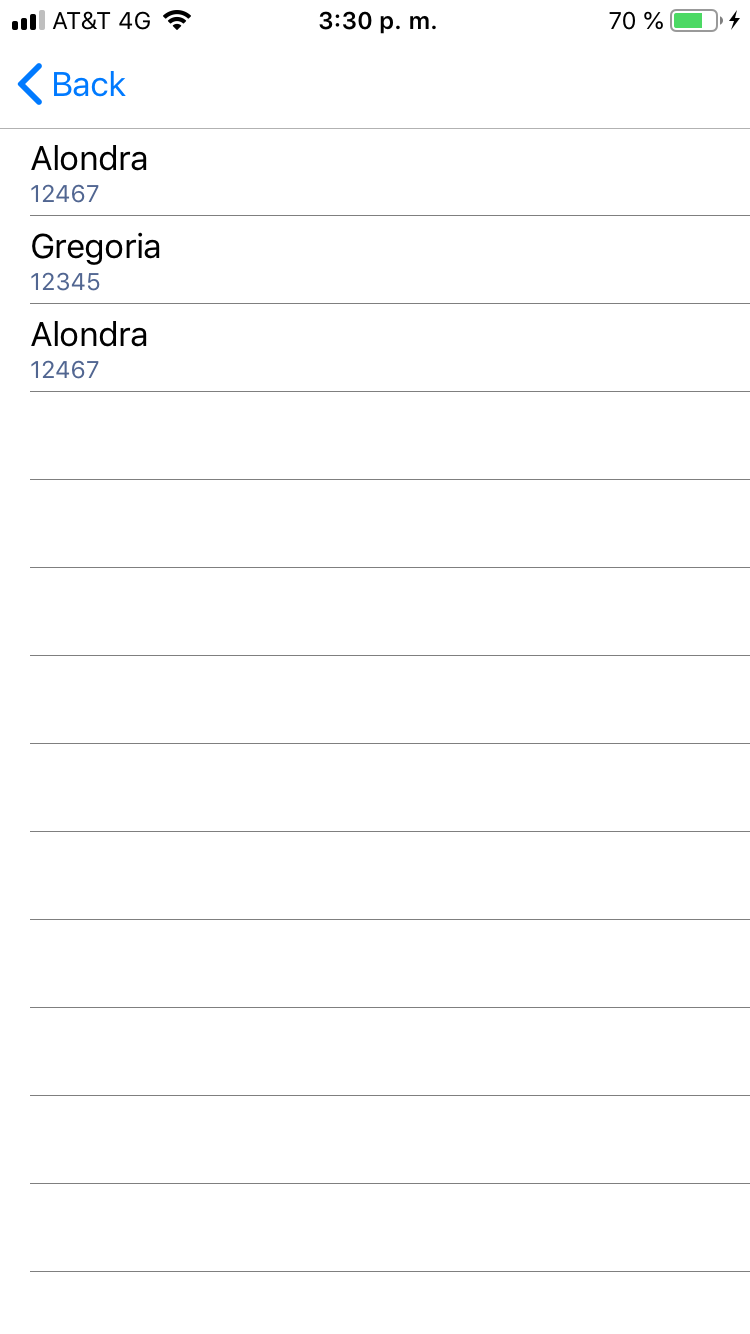
\includegraphics[height=0.4\textheight]{Doctor/ConsultarPacientes/images/Pacientes}
			\caption{Pacientes}
			\label{fig:Pacientes}
		\end{center}
	\end{figure}
	
	\item Se mostrará la pantalla \textbf{Información del Paciente}.
	\newpage
	\begin{figure}[!htbp]			
		\hypertarget{fig:infoPacientes}{\hspace{1pt}}
		\begin{center}
			\includegraphics[height=0.4\textheight]{images/Iconos/Advertencia}
			\caption{Información del Paciente}
			\label{fig:infoPacientes}
		\end{center}
	\end{figure}

	\item Consulta la información del tratamiento del paciente.


\end{enumerate}

